\usepackage{shared/cs45}
\usepackage{tikz}
\usetikzlibrary{graphs}
\tikzset{>=latex}

\title{CS 45, Lecture 8}
\subtitle{Version Control}
\date{Winter 2023}
\author{Akshay Srivatsan, Ayelet Drazen, Jonathan Kula}

\newcommand{\var}[1]{\texttt{\$#1}}
\newcommand{\cmd}[1]{\mintinline{shell}{#1}}

\begin{document}

\maketitle

\frame{\titlepage}

\begin{frame}
  \frametitle{Outline}
  \tableofcontents[hidesubsections]
\end{frame}

\section{Review}

\begin{frame}{Computer Networks}
  Last lecture, we saw:
  \begin{itemize}
    \item How computers can use a network to talk to each other
    \item How information gets sent from one place to another over the internet
  \end{itemize}
  \pause

  In this lecture, we will see:
  \begin{itemize}
    \item How to safely store your files (code or text)
    \item How to collaborate on files with others over the internet
    \item \alert{How to avoid losing all your homework!}
  \end{itemize}
\end{frame}

\begin{frame}{Files}
  \begin{itemize}
    \item Many of the files you work with will be text:
      \pause
      \begin{itemize}
        \item Source Code
        \item Documentation
        \item Markup Files
      \end{itemize}
    \pause
    \item As you change these files over time, you'll eventually want some way
      to keep track of different \enquote{versions} of the file.
    \pause
    \item What we need is a \enquote{version control system}.
  \end{itemize}
\end{frame}

\section{Version Control}
\subsection{Version Control Systems}

\begin{frame}{Version Control Systems}
  \begin{itemize}
    \item A \textsc{version control system} (VCS) is a piece of software which
      manages different versions of your files and folders for you.
    \pause
    \item A good VCS will let you look at old versions of files and restore
      files (or information) which you might have accidentally deleted.
    \pause
    \item You've seen these before!
  \end{itemize}
\end{frame}

\begin{frame}{Version Control Systems}
  \vspace{-1em}
  \begin{center}
    \includegraphics[width=0.35\textwidth]{images/google-docs-vcs.png}
    \includegraphics[width=0.35\textwidth]{images/assign2-versions.png}
  \end{center}
\end{frame}

\begin{frame}{Version Control Systems}
  A good version control system:
  \begin{itemize}
    \item Will store many versions of your files \pause

    \item Will let you \enquote{revert} a file (or a part of a file) to an
      older version \pause

    \item Will track the order of different versions \pause

    \item Will ensure each \enquote{version} is neither too big nor too small
      \pause
  \end{itemize}
  A great version control system:
  \begin{itemize}
    \item Will let you collaborate on files with other people \pause

    \item Will combine the different versions of the files produced by
      different people sanely
  \end{itemize}
\end{frame}

\subsection{Comparison of VCSs}

There are many different ways to set up a version control system.  Let's see
the pros and cons of some of the more common ones.

\begin{frame}{Google Docs}
  Google Docs automatically keeps track of file history in a basic VCS.

  Pros:
  \begin{itemize}
    \item Great for rich text
    \item Allows real-time collaboration
    \item Saved on the cloud automatically\mode<article>{\footnote{Stay tuned for our lecture on the cloud!}}
  \end{itemize}

  Cons:
  \begin{itemize}
    \item Bad for plain text (especially code)
    \item Requires an internet connection
    \item Only supports a single \enquote{current} version of a single file
  \end{itemize}

  \mode<article>{
    You might wonder why you'd ever want multiple \enquote{current} versions of
    a file.  One example is when we are planning out this class---we have
    multiple ideas for each part of an assignment, and try to flesh them out
    enough to see what works and what doesn't.  It would be nice if we could
    have multiple, equally-valid, versions of the assignment at the same time,
    but right now the only way to do that is to copy the file.
  }
\end{frame}

\begin{frame}{Copying Files}
  You can make a bunch of copies of files or folders with \cmd{cp} as a simple
  form of version control.  You can compare versions with \cmd{diff}.

  Pros:
  \begin{itemize}
    \item Works on either rich or plain text (or anything else)
    \item It's simple and makes it easy to move data between versions
  \end{itemize}

  Cons:
  \begin{itemize}
    \item It's messy and a lot of manual work
    \item It's hard to tell what the relationship between different versions
      is
    \item It takes a lot of hard drive space
  \end{itemize}
\end{frame}

\begin{frame}{Zip Files}
  Instead of just \cmd{cp}ing folders, we could bundle them up into a Zip file
  (a single file which can be \enquote{unzipped} into a folder).

  Pros:
  \begin{itemize}
    \item Tracks versions for an entire folder at once
    \item Easy to share a version with someone else (email)
  \end{itemize}

  Cons:
  \begin{itemize}
    \item It's still a lot of manual work
    \item It's hard to tell what the relationship between different versions
      is
    \item It's hard to extract a single file from an old version
  \end{itemize}
\end{frame}

\begin{frame}{Zip Files++}
  \begin{itemize}
    \item
      What if we had a tool which did all this zip file stuff automatically?
      \pause
    \item
      We could tell it to take a \enquote{snapshot} of a directory, and it
      would save all the changes in it.\mode<article>{\footnote{Or, even better,
      we could tell it \textit{which} files to save in the snapshot.
      Everything else stays as it was in the previous snapshot.}}
      \pause
    \item
      We could ask it to recover an old version of a specific file, or to reset
      everything to an old version to \enquote{undo} our work.
      \pause
    \item
      The tool could track the relationships between different versions, so we
      can have multiple \enquote{current} versions at the same time.
      \pause
    \item
      If we want to combine different versions, the tool can automatically do
      it for us (instead of us copying and pasting the parts together).
  \end{itemize}
\end{frame}

\begin{frame}{Git}
  \vspace{-0.5em}
  \cmd{git} is a version control system which tracks \enquote{commits}
  (snapshots) of files in a \textsc{repository}.
  \pause
  \begin{itemize}
    \item
      Git stores old versions of files in a hidden folder (\cmd{.git}), and
      automatically manages them.
      \pause
    \item
      We can tell Git to keep track of certain files, and tell it when to take
      a snapshot.
      \pause
    \item
      We can ask Git to go back to an old snapshot (even for a single file).
      \pause
    \item
      We can ask Git to keep track of who's working on what, so multiple people
      can work on different things without conflicting.
      \pause
    \item
      If we want to combine multiple people's work, we can ask Git to
      automatically merge them together. If it can't for some reason, it'll ask
      us to manually merge them.
  \end{itemize}
\end{frame}

There are several other version control systems in use, but Git is by far the
most popular.  Different companies sometimes decide to use different VCSes for
various reasons; for example, Facebook/Meta uses a version of Mercurial
(another VCS) they call \enquote{Sapling}.  However, these different VCSes are
conceptually very similar, so moving from one to another is pretty easy.

\section{Git}

\subsection{Linear History}
\begin{frame}{Basic Workflow}
  \vspace{-0.5em}
  The simplest way to use git is the \enquote{linear} workflow, which is the
  same way you'd use Google Docs:
  \pause
  \begin{enumerate}
    \item \cmd{git init} to enable Git in a certain directory 
      \pause
    \item \cmd{git add} any files you want Git to \enquote{track}
      \pause
    \item \cmd{git commit} the currently \enquote{staged} changes to save a
      snapshot
      \pause
    \item make changes to your files
      \pause
    \item \cmd{git add} the changed files to \enquote{stage} them again
      \pause
    \item Repeat from 3
  \end{enumerate}

  You can use \cmd{git log} to see your commit history, and use \cmd{git
  status} to see the current state of staged/unstaged/untracked changes.
\end{frame}

Before you do anything in Git, you should tell Git who you are:
\begin{minted}{shell}
git config --global user.name "<YOUR FULL NAME>"
git config --global user.email "<YOUR PUBLIC EMAIL ADDRESS>"
\end{minted}

Note that these configuration values will be permanently baked into any commits
you make, so other people may be able to see them.  Use a pseudonym or a
pseudonymous email address if you don't want to publish your information; see
\href{https://docs.github.com/en/account-and-profile/setting-up-and-managing-your-personal-account-on-github/managing-email-preferences/setting-your-commit-email-address}{the
GitHub Docs} for more info.

\begin{frame}{Basic Workflow}{Demo}
  Let's practice how to:
  \begin{itemize}
    \item Create a new Git repository
    \item Commit a new file
    \item Commit changes to files
    \item Revert commits
    \item Look at an old version of a file
    \item Compare two versions of files
    \item See your commit history
  \end{itemize}
\end{frame}

\subsection{Branching Workflow}
\begin{frame}{Branching Workflow}
  We can also split our \enquote{repo} into multiple \textsc{branches}, which
  are like alternate versions of a folder.  This means different people can
  work on different things without interfering with one another.
  \pause
  \begin{enumerate}
    \item Make sure your repository is \enquote{clean} (i.e., you have no uncommitted changes).
      \pause
    \item \cmd{git checkout -b <branch>} to create a new branch and move to it;
      at this point, the new branch will be identical to the old one.
    \item Make changes, \cmd{git add}, \cmd{git commit} as usual
    \item \cmd{git checkout} to switch between branches
  \end{enumerate}
\end{frame}

\subsection{Combining Branches}
\begin{frame}{Branching Workflow}{Combining Branches}
  Now that we have multiple branches, we probably want to join them back
  together at some point.

  There are several ways to do this:
  \begin{itemize}
    \item \cmd{git merge} two branches into one
    \item \cmd{git merge --fast-forward} a long branch onto a shorter version
      of itself
    \item \cmd{git rebase} one branch onto another branch
    \item \cmd{git cherry-pick} a specific commit from one branch to another
  \end{itemize}
\end{frame}

\begin{frame}{Branching Workflow}{Fast Forwarding}
  The simplest case of \textsc{merging} is called \textsc{fast-forwarding}.
  \mode<presentation>{\vfill}
  \begin{center}
    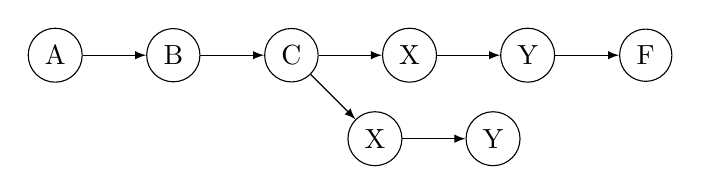
\begin{tikzpicture}[node distance = {15mm}, commit/.style = {draw, circle}]
      \node[commit] (A) {A};
      \node[commit] (B) [right of=A] {B};
      \node[commit] (C) [right of=B] {C};
      \draw[->] (A) to (B);
      \draw[->] (B) to (C);
      \pause
      \uncover<2>{
        \node[commit] (X) [below right of=C] {X};
        \draw[->] (C) to (X);
        \node[commit] (Y) [right of=X] {Y};
        \draw[->] (X) to (Y);
      }
      \uncover<3-> {
        \node[commit] (X2) [right of=C] {X};
        \draw[->] (C) to (X2);
        \node[commit] (Y) [right of=X2] {Y};
        \draw[->] (X2) to (Y);
      }
      \pause
      \pause
      \node[commit] (F) [right of=Y] {F};
      \draw[->] (Y) to (F);
    \end{tikzpicture}
  \end{center}
\end{frame}

Assume there was a main branch containing A and B.  We then created a new
branch based on B, containing X and Y.  Merging the main branch and our new
branch is easy---our new branch is just a longer version of the main branch, so
we can \enquote{fast-forward} the main branch to catch up.  We can then commit
F on the main branch, based on Y.

\begin{frame}{Branching Workflow}{Merging}
  \textsc{Merging} (in general) creates a \textsc{merge commit} to join the two
  branches.
  \mode<presentation>{\vfill}
  \begin{center}
    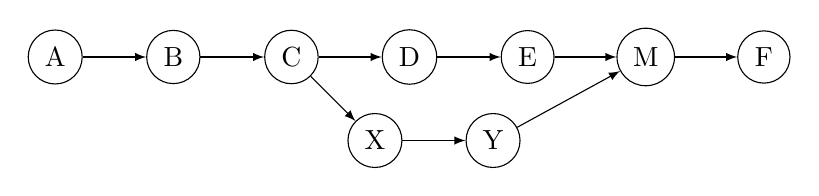
\begin{tikzpicture}[node distance = {15mm}, commit/.style = {draw, circle}]
      \node[commit] (A) {A};
      \node[commit] (B) [right of=A] {B};
      \node[commit] (C) [right of=B] {C};
      \draw[->] (A) to (B);
      \draw[->] (B) to (C);
      \pause
      \node[commit] (X) [below right of=C] {X};
      \draw[->] (C) to (X);
      \node[commit] (Y) [right of=X] {Y};
      \draw[->] (X) to (Y);
      \pause
      \node[commit] (D) [right of=C] {D};
      \draw[->] (C) to (D);
      \node[commit] (E) [right of=D] {E};
      \draw[->] (D) to (E);
      \pause
      \node[commit] (M) [right of=E] {M};
      \draw[->] (Y) to (M);
      \draw[->] (E) to (M);
      \pause
      \node[commit] (F) [right of=M] {F};
      \draw[->] (M) to (F);
    \end{tikzpicture}
  \end{center}
\end{frame}

In this case, assume as before that we had a main branch containing A and B. We
created a new branch and added X and Y.  However, while we were doing that,
someone else added D and E to the main branch.  Our branch has now
\textsc{diverged} from the main branch; we both have different, possibly
contradictory ideas of what the \enquote{real} state is.  We fix this by
creating a \textsc{merge commit} M, which contains a combination of E and Y; if
E and Y were contradictory, Git will ask the user to resolve the \textsc{merge
conflict} by picking which version to keep.  Now we're back to a single \enquote{real} version M, so we can add F on the end.

\begin{frame}{Branching Workflow}{Rebasing}
  \textsc{Rebasing} moves the \enquote{base} of a branch to be a different
  commit.
  \uncover<7>{%
    \alert{%
      \textsc{Rebasing} edits Git's history to make \textsc{fast-forwarding}
      possible.
    }
  }
  \mode<presentation>{\vfill}
  \begin{center}
    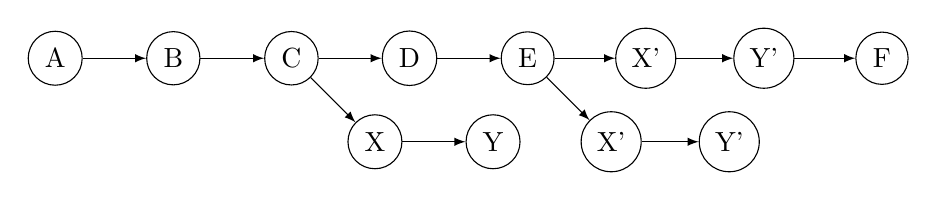
\begin{tikzpicture}[node distance = {15mm}, commit/.style = {draw, circle}]
      \node[commit] (A) {A};
      \node[commit] (B) [right of=A] {B};
      \node[commit] (C) [right of=B] {C};
      \draw[->] (A) to (B);
      \draw[->] (B) to (C);
      \pause
      \only<1-3> {
        \node[commit] (X) [below right of=C] {X};
        \draw[->] (C) to (X);
        \node[commit] (Y) [right of=X] {Y};
        \draw[->] (X) to (Y);
      }
      \pause
      \node[commit] (D) [right of=C] {D};
      \draw[->] (C) to (D);
      \node[commit] (E) [right of=D] {E};
      \draw[->] (D) to (E);
      \pause
      \uncover<4> {
        \node[commit] (X2) [below right of=E] {X'};
        \draw[->] (E) to (X2);
        \node[commit] (Y2) [right of=X2] {Y'};
        \draw[->] (X2) to (Y2);
      }
      \pause
      \node[commit] (X2) [right of=E] {X'};
      \draw[->] (E) to (X2);
      \node[commit] (Y2) [right of=X2] {Y'};
      \draw[->] (X2) to (Y2);
      \pause
      \node[commit] (F) [right of=Y2] {F};
      \draw[->] (Y2) to (F);
      \pause
    \end{tikzpicture}
  \end{center}
\end{frame}

Again assume that we had a main branch containing A and B, from which we
created a new branch and added X and Y.  Once again, someone else added D and E
to the main branch while we weren't looking.  However, this time, we want to
maintain the illusion of \enquote{linear history}; the idea that every version
has exactly one predecessor and one successor.  This is obviously not true in
this case---the commit C has two successors---so we \enquote{rebase} our
branch.  This creates a new commit X' which combines X and E, and a new commit
Y' which combines Y and X'.  However, if you look at the Git history, you never
see a reference to the original X or Y; for all practical purposes, X and Y
never existed.  Now we're back to the fast-forward case; our branch is a longer
version of \cmd{main}, so we can fast-forward \cmd{main} to include X' and Y'.
Now we can commit a new F based on Y'; if anyone in the future ever looks at
the repository, it'll look like everything up to F was a linear, non-branching,
sequence of changes.


\begin{frame}{Branching Workflow}{Cherry-Picking}
  \textsc{Cherry-picking} copies a \textit{single commit} from one branch to
  another branch. %
  \uncover<7->{%
    \alert {%
      \textsc{Cherry-picking} and rebasing is a good way to move a single
      commit from one branch to another.
    }
  }
  \mode<presentation>{\vfill}
  \begin{center}
    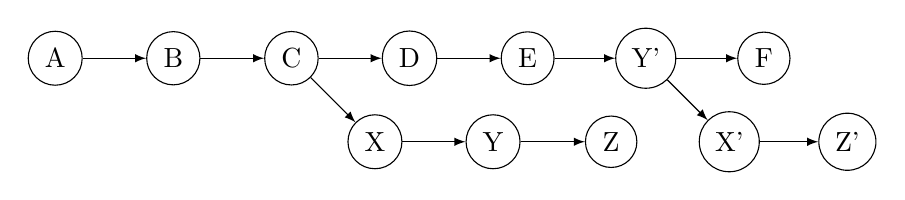
\begin{tikzpicture}[node distance = {15mm}, commit/.style = {draw, circle}]
      \node[commit] (A) {A};
      \node[commit] (B) [right of=A] {B};
      \node[commit] (C) [right of=B] {C};
      \draw[->] (A) to (B);
      \draw[->] (B) to (C);
      \pause
      \uncover<2-5> {
        \node[commit] (X) [below right of=C] {X};
        \draw[->] (C) to (X);
        \node[commit] (Y) [right of=X] {Y};
        \draw[->] (X) to (Y);
        \node[commit] (Z) [right of=Y] {Z};
        \draw[->] (Y) to (Z);
      }
      \pause
      \node[commit] (D) [right of=C] {D};
      \draw[->] (C) to (D);
      \node[commit] (E) [right of=D] {E};
      \draw[->] (D) to (E);
      \pause
      \node[commit] (Y2) [right of=E] {Y'};
      \draw[->] (E) to (Y2);
      \pause
      \node[commit] (F) [right of=Y2] {F};
      \draw[->] (Y2) to (F);
      \pause
      \node[commit] (X2) [below right of=Y2] {X'};
      \draw[->] (Y2) to (X2);
      \node[commit] (Z2) [right of=X2] {Z'};
      \draw[->] (X2) to (Z2);
      \pause
    \end{tikzpicture}
  \end{center}
\end{frame}

Sometimes we want to grab a specific change from another branch, without
merging or rebasing the entire branch.  This is a use case for
\enquote{cherry-picking}, selecting a specific commit to copy into another
branch.  In this case, assume a similar setup to the previous cases---a main
branch containing A, B, C, D, and E, and a new branch containing A, B, X, and
Y, and Z.  We're on the main branch at E, and we realize we need something that
was added in commit Y, but we \textbf{don't} want to include commit X or commit
Z.  We can't literally just copy Y onto our main branch, since it depends on X
and doesn't include anything from D or E, so we create a new commit Y'.  Y' is
like a mashup of Y and E, but without any of the stuff from X.  Now we can
commit F based on Y', and F will contain no references to X or Z.

Note that this can get weird if you later do a merge---Y and Y' will both be in
your history!  If you cherry-pick commits like this, you probably want to do a
rebase to make your history less confusing; in this case we could rebase the
new branch onto Y', creating a new X' and Z', which would effectively erase the original X, Y, and Z from the new branch.

\begin{frame}{Branching Workflow}{When to merge/rebase/cherry-pick?}
  \begin{itemize}
    \item \textbf{fast-forward} when possible (\cmd{git merge --ff-only}).
    \item \textbf{rebase and then fast-forward} if possible, i.e., if you're
      the only one working on the branch; \textbf{never} rebase a branch other
      people are using (\cmd{git rebase} and \cmd{git merge --ff-only}).
    \item \textbf{merge} if neither of the above are possible (\cmd{git
      merge}).
    \item \textbf{cherry-pick} if you want to copy a specific commit to another
      branch (\cmd{git cherry-pick})\footnote{This is pretty rare, I've only
      used it a handful of times.}.
  \end{itemize}
\end{frame}

Some projects insist upon having linear history in \cmd{main}, which means any
merge commits will be rejected.  In this case, you should first \cmd{rebase}
your changes onto the most recent \cmd{main}, then \cmd{merge --ff-only} to
fast-forward \cmd{main} to include your changes.  Most projects are okay with
merge commits, so you can just use \cmd{merge} and forget that \cmd{rebase}
ever existed.

\begin{frame}{Branching Workflow}{Branching Demo}
  Let's practice how to:
  \begin{itemize}
    \item Split our repository into two branches
    \item Switch between branches
    \item Make commits on either branch
    \item Merge two branches together
  \end{itemize}
\end{frame}

\begin{frame}{To Be Continued\textellipsis}
  We'll pick back up with merge conflict resolution and collaboration in Lecture 9.

  Some commands which came up during class:
  \begin{description}
    \item[\texttt{git checkout}:] essentially means \enquote{move to a
      different commit}; doesn't change your git history
    \item[\texttt{git reset}:] \enquote{resets} the entire repository to the
      way it was in an old commit (and changes git history to match)
    \item[\texttt{git revert}:] \enquote{undoes} a specific old commit by
      creating a new commit that does the opposite
  \end{description}

  Note that, even though Git commits are technically versions, Git's commands
  often operate on the \textit{changes} between versions.
\end{frame}

You can view all your active branches with \texttt{git branch}, and delete
branches with \texttt{git branch -d}.  Remember that a \enquote{branch} is
basically just a named version of a file; \enquote{main} is typically the
official version, while other branches are so-called \enquote{feature branches}
where different people can experiment with adding different things.  Generally
a feature branch should be \enquote{owned} by a single person to avoid
conflicts (only that person should ever change that branch).

One last thing: git has separate man pages for each subcommand, since they're
each so complicated they need their own docs.  For example, the man page for
\cmd{git commit} can be viewed using \cmd{man git-commit}.

\end{document}
